\documentclass[UTF8,aspectratio=169]{ctexbeamer}
\usetheme[maxplus,default]{sjtubeamer}
\graphicspath{{img/}}
\usepackage{float}
% \usepackage{parskip} % parskip has no effect on columns
\usepackage{gbt7714}
\begin{document}
    \title{COVID Insights}
    \subtitle{疫情可视化案例分析}
    \author{李子龙}
    \institute[Copyright \copyright{} 2020 Microsoft Corporation.]{}
    \maketitle

    \begin{frame}
        \frametitle{简介}
        \begin{columns}
            \begin{column}{0.4\textwidth}
        微软亚洲研究院(Microsoft Research Lab -- Asia, MSRA)于 2020 年推出了 COVID Insights 网站\footnotemark,基于计算生物学、数据科学等领域的研究,以可视化可交互式从流行病学、病毒学、研究趋势三个方面分析新冠疫情的相关情况。
            \end{column}
            \begin{column}{0.6\textwidth}
                \begin{figure}[H]
                    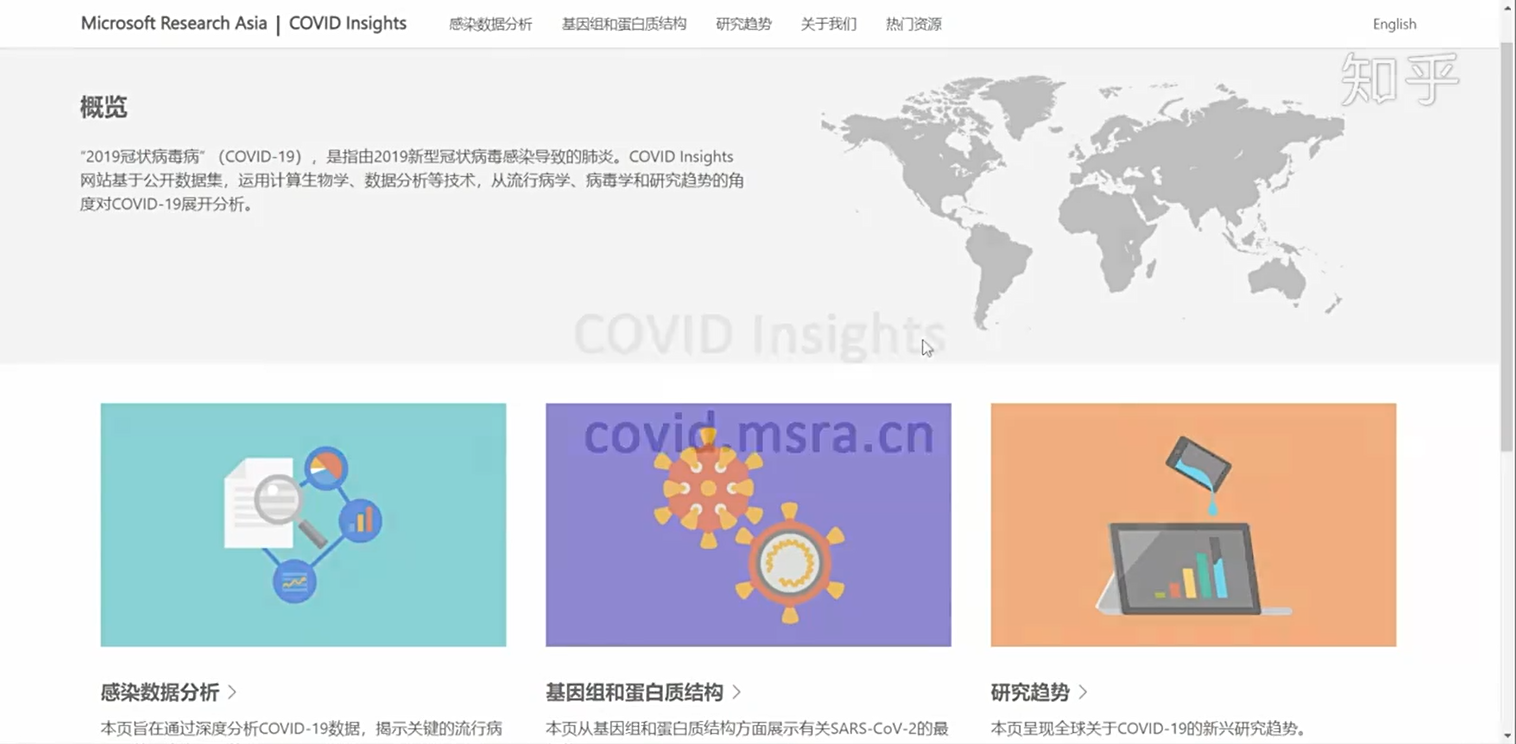
\includegraphics[width=\linewidth]{intro}
                \caption{概览\cite{msracn}}\label{fig:intro}
                \end{figure}
            \end{column}
        \end{columns}
        \footnotetext{网址为 \href{https://covid.msra.cn}{\texttt{covid.msra.cn}},现在已经关闭,根据当时的印象以及报道\cite{msracn}进行介绍。}
    \end{frame}

    \begin{frame}
        \frametitle{流行病学}
        \begin{columns}
            \begin{column}{0.4\textwidth}
                \only<1>{通过分析不同国家和地区的确诊病例与死亡病例数据,来得到该国家或地区在数据趋势上发展相似的另一方,如图 \ref{fig:trend} 所示。}

                \only<2>{\paragraph{优点} 这种对趋势对比的可视化有助于我们大致预测该地区下一段时间的趋势情况,通过显示相似区间以在视觉上产生说服力。

                \paragraph{缺点} 由于每个国家和地区的医疗卫生水平不同,这种趋势比较可能具有误导性,有可能让观者直接接受这种可信度不太高的结论。
                }
            \end{column}
            \begin{column}{0.6\textwidth}
                \begin{figure}[H]
                    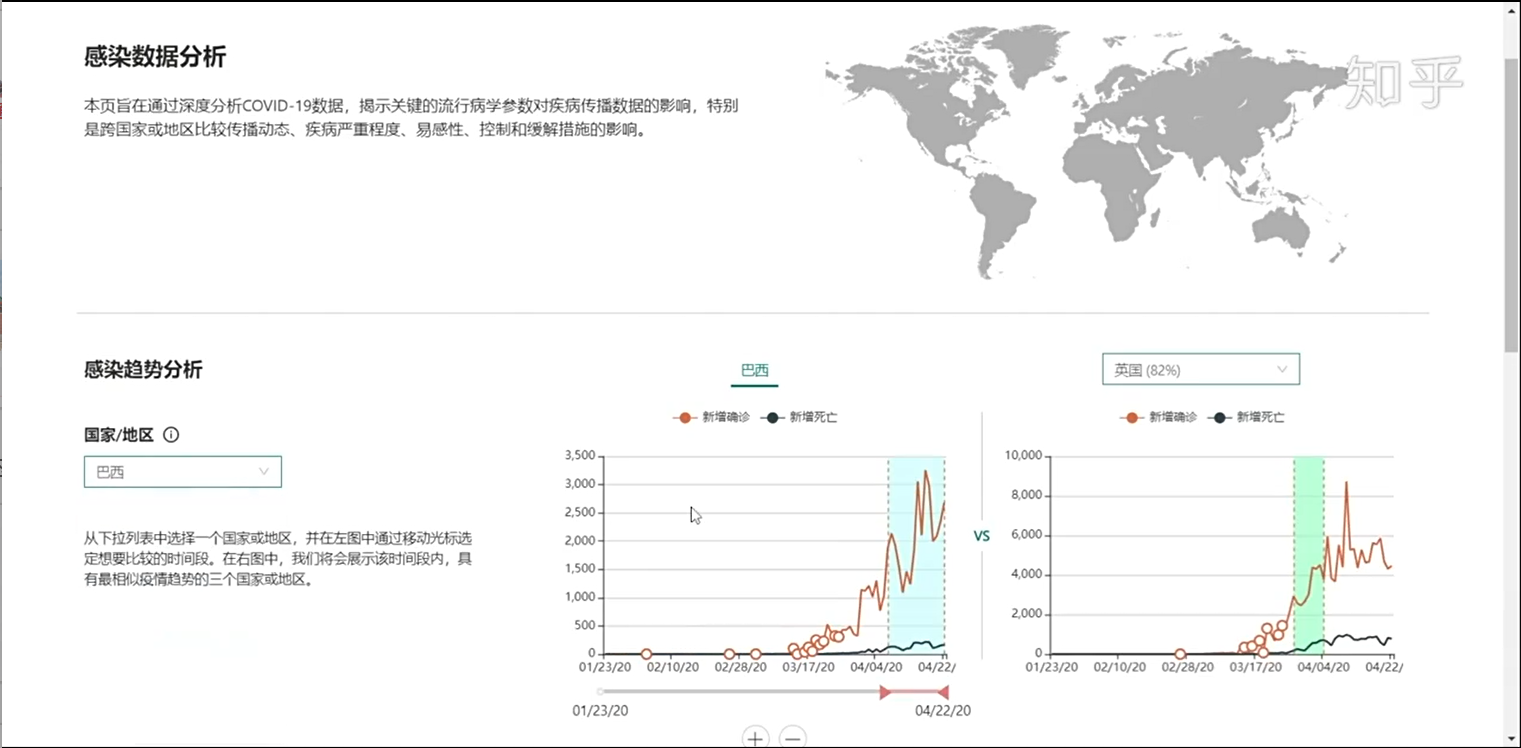
\includegraphics[width=\linewidth]{trend}
                    \caption{趋势对比\cite{msracn}}\label{fig:trend}
                \end{figure}
            \end{column}
        \end{columns}
    \end{frame}

    \begin{frame}
        \frametitle{病毒学}
        \framesubtitle{基因组变异}
        \begin{columns}
            \begin{column}{0.4\textwidth}
                \only<1>{如图 \ref{fig:genome} 所示,从左到右依次是选定对应的 RNA 序列、查看该区间的氨基酸多样性信息、该位置的不同氨基酸种类的病毒序列数目趋势。右上角是选定相关区域的病毒变异种的占比情况。}

                \only<2>{\paragraph{优点} 以地图饼状图的形式展示了哪种病毒变异种在占主导趋势,以三个相互关联的统计图直观地显示数据之间的关系,看清楚变异趋势。

                \paragraph{缺点} 下面三张图的联系仍然没有那么直观,外行只能看到某种感觉,可读性上有待加强。
                }
            \end{column}
            \begin{column}{0.6\textwidth}
                \begin{figure}[H]
                    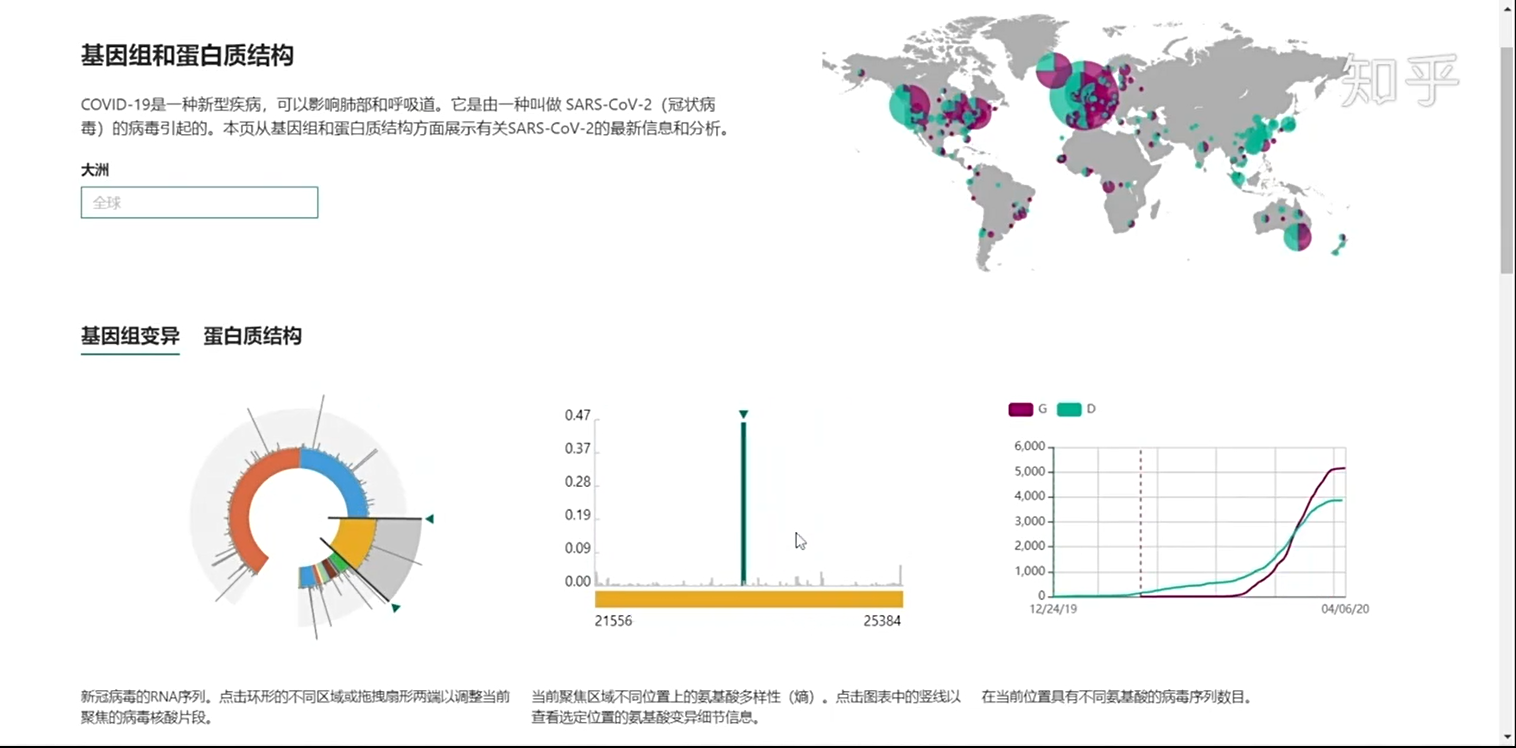
\includegraphics[width=\linewidth]{genome}
                    \caption{基因组变异\cite{msracn}\label{fig:genome}}
                \end{figure}
            \end{column}
        \end{columns}
    \end{frame}

    \begin{frame}
        \frametitle{病毒学}
        \framesubtitle{蛋白质结构}
        \begin{columns}
            \begin{column}{0.4\textwidth}
                \only<1>{如图 \ref{fig:virus} 所示,展示了病毒的蛋白质结构。}

                \only<2>{\paragraph{优点} 以一种三维可视化的方式对病毒的情况进行科普,形象易懂,模型精致。

                    \paragraph{缺点} 病毒模型仍然是静态图像,可以改为三维可交互性展示,方便观者拥有更多的空间思考。
                }
            \end{column}
            \begin{column}{0.6\textwidth}
                \begin{figure}[H]
                    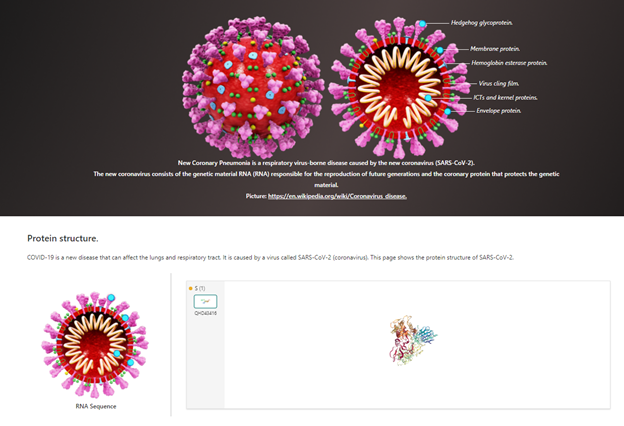
\includegraphics[width=\linewidth]{virus}
                    \caption{蛋白质结构\cite{msracn}\label{fig:virus}}
                \end{figure}
            \end{column}
        \end{columns}
    \end{frame}

    \begin{frame}
        \frametitle{研究趋势}
        \begin{columns}
            \begin{column}{0.4\textwidth}

                \only<1>{
                如图 \ref{fig:research} 所示,采用词云可视化当前研究趋势热点,并提供了一个可拖拽的时间拉杆,显示热点变化。
                }
                
                \only<2>{
                \paragraph{优点} 通过词云展示热点情况,是一种流行的统计展示手法,简洁明了,可视性强。

                \paragraph{缺点} 词云只是为了符合某种特殊的形状设计的,并不能很好地展现词语之间的联系,为了美观在这方面有了一些妥协。同一词语在时间趋势的动态变化也很难体现。
                }
            \end{column}
            \begin{column}{0.6\textwidth}
                \begin{figure}[H]
                    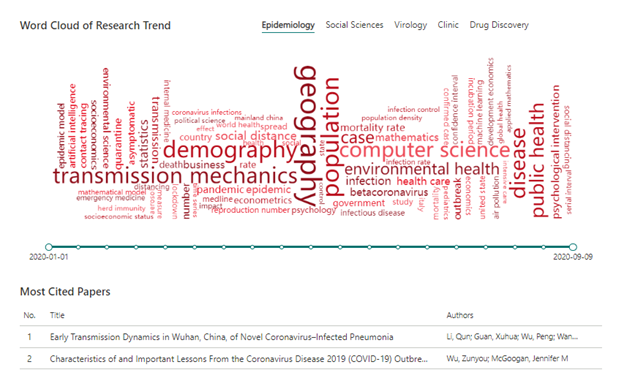
\includegraphics[width=\linewidth]{research}
                    \caption{研究趋势\cite{msraen}}\label{fig:research}
                \end{figure}
            \end{column}
        \end{columns}
    \end{frame}

    \begin{frame}
        \frametitle{参考}
        \bibliography{ref}
        \vfill
        Built by \href{https://github.com/sjtug/SJTUBeamer}{SJTUBeamer}.

        Copyright \copyright{} 2020 Microsoft Corporation.
    \end{frame}

    \makebottom
\end{document}